%\documentclass[14pt, handout]{beamer} 		% for print 
\documentclass[12pt]{beamer} 					% for projector
%\documentclass[12pt, a4paper]{article} 

\usepackage{fontspec} % Font selection for XeLaTeX; see fontspec.pdf. 
\usepackage{xeCJK}	% 中文使用 XeCJK,利用 \setCJKmainfont 定義中文內文、粗體與斜體的字型
\defaultfontfeatures{Mapping=tex-text} % to support TeX conventions like ``---''
\usepackage{xunicode} % Unicode support for LaTeX character names(accents, European chars, etc)
\usepackage{xltxtra} 				% Extra customizations for XeLaTeX
\usepackage{amsmath, amssymb}
\usepackage{enumerate}
\usepackage{graphicx,subfig,float,wrapfig} % support the \includegraphics command and options
\usepackage[outercaption]{sidecap} %[options]=[outercaption], [innercaption], [leftcaption], [rightcaption]
\usepackage{array, booktabs}
\usepackage{color, xcolor}
\usepackage{longtable}
\usepackage{colortbl}                          				
\usepackage{listings}						% 直接將 latex 碼轉換成顯示文字
\usepackage[parfill]{parskip} 				% 新段落前加一空行,不使用縮排
\usepackage[left=1.5in,right=1in,top=1in,bottom=1in]{geometry} 
\usepackage{url}

%-----------------------------------------------------------------
%  中英文內文字型設定
\setCJKmainfont							% 設定中文內文字型
	[
		BoldFont=Microsoft YaHei	    %定義粗體的字型(Win)
%		BoldFont=蘋果儷中黑	    		%定義粗體的字型(Mac)
	]
	{新細明體}						% 設定中文內文字型(Win)
%	{宋體-繁}							% 設定中文內文字型(Mac)	
\setmainfont{Times New Roman}		% 設定英文內文字型
\setsansfont{Arial}					% 無襯字字型 used with {\sffamily ...}
%\setsansfont[Scale=MatchLowercase,Mapping=tex-text]{Gill Sans}
\setmonofont{Courier New}			% 等寬字型 used with {\ttfamily ...}
%\setmonofont[Scale=MatchLowercase]{Andale Mono}
% 其他字型(隨使用的電腦安裝的字型不同,用註解的方式調整(打開或關閉))
% 英文字型
\newfontfamily{\E}{Calibri}				
\newfontfamily{\A}{Arial}
\newfontfamily{\C}[Scale=0.9]{Arial}
\newfontfamily{\R}{Times New Roman}
\newfontfamily{\TT}[Scale=0.8]{Times New Roman}
% 中文字型
\newCJKfontfamily{\MB}{微軟正黑體}				% 等寬及無襯線字體 Win
%\newCJKfontfamily{\MB}{黑體-繁}				% 等寬及無襯線字體 Mac
\newCJKfontfamily{\SM}[Scale=0.8]{新細明體}	% 縮小版(Win)
%\newCJKfontfamily{\SM}[Scale=0.8]{宋體-繁}	% 縮小版(Mac)
\newCJKfontfamily{\K}{標楷體}                	% Windows下的標楷體
%\newCJKfontfamily{\K}{楷體-繁}               	% Mac下的標楷體
\newCJKfontfamily{\BB}{Microsoft YaHei}		% 粗體 Win
%\newCJKfontfamily{\BB}{蘋果儷中黑}		% 粗體 Mac
% 以下為自行安裝的字型:CwTex 組合
%\newCJKfontfamily{\CF}{cwTeX Q Fangsong Medium}	% CwTex 仿宋體
%\newCJKfontfamily{\CB}{cwTeX Q Hei Bold}			% CwTex 粗黑體
%\newCJKfontfamily{\CK}{cwTeX Q Kai Medium}   	% CwTex 楷體
%\newCJKfontfamily{\CM}{cwTeX Q Ming Medium}		% CwTex 明體
%\newCJKfontfamily{\CR}{cwTeX Q Yuan Medium}		% CwTex 圓體
%-----------------------------------------------------------------------------------------------------------------------
\XeTeXlinebreaklocale "zh"             		%這兩行一定要加,中文才能自動換行
\XeTeXlinebreakskip = 0pt plus 1pt     		%這兩行一定要加,中文才能自動換行
%-----------------------------------------------------------------------------------------------------------------------
\newcommand{\cw}{\texttt{cw}\kern-.6pt\TeX}	% 這是 cwTex 的 logo 文字
\newcommand{\imgdir}{images/}				% 設定圖檔的目錄位置
\renewcommand{\tablename}{表}	% 改變表格標號文字為中文的「表」(預設為 Table)
\renewcommand{\figurename}{圖}% 改變圖片標號文字為中文的「圖」(預設為 Figure)

% 設定顏色 see color Table: http://latexcolor.com
\definecolor{slight}{gray}{0.9}				
\definecolor{airforceblue}{rgb}{0.36, 0.54, 0.66} 
\definecolor{arylideyellow}{rgb}{0.91, 0.84, 0.42}
\definecolor{babyblue}{rgb}{0.54, 0.81, 0.94}
\definecolor{cadmiumred}{rgb}{0.89, 0.0, 0.13}
\definecolor{coolblack}{rgb}{0.0, 0.18, 0.39}
\definecolor{beaublue}{rgb}{0.74, 0.83, 0.9}
\definecolor{beige}{rgb}{0.96, 0.96, 0.86}
\definecolor{bisque}{rgb}{1.0, 0.89, 0.77}
\definecolor{gray(x11gray)}{rgb}{0.75, 0.75, 0.75}
\definecolor{limegreen}{rgb}{0.2, 0.8, 0.2}
\definecolor{splashedwhite}{rgb}{1.0, 0.99, 1.0}

%---------------------------------------------------------------------
% 映出程式碼 \begin{lstlisting} 的內部設定
\lstset
{	language=[LaTeX]TeX,
    breaklines=true,
    %basicstyle=\tt\scriptsize,
    basicstyle=\tt\normalsize,
    keywordstyle=\color{blue},
    identifierstyle=\color{black},
    commentstyle=\color{limegreen}\itshape,
    stringstyle=\rmfamily,
    showstringspaces=false,
    %backgroundcolor=\color{splashedwhite},
    backgroundcolor=\color{slight},
    frame=single,							%default frame=none 
    rulecolor=\color{gray(x11gray)},
    framerule=0.4pt,							%expand outward 
    framesep=3pt,							%expand outward
    xleftmargin=3.4pt,		%to make the frame fits in the text area. 
    xrightmargin=3.4pt,		%to make the frame fits in the text area. 
    tabsize=2				%default :8 only influence the lstlisting and lstinline.
}

% 映出程式碼 \begin{lstlisting} 的內部設定 for Python codes
%\lstset{language=Python}
%\lstset{frame=lines}
%\lstset{basicstyle=\SCP\normalsize}
%\lstset{keywordstyle=\color{blue}}
%\lstset{commentstyle=\color{airforceblue}\itshape}
%\lstset{backgroundcolor=\color{beige}} % disable geometry for Beamer
\input{preamble_addon_Beamer}
%-----------------------------------------------------------------------------------------------------------------------
% 文章開始

\title[統計計算]{{\MB 統計應用數學與計算}}  % 從編譯好的結果,看看這幾個字出現在什麼地方
\author[CC Wang]{汪群超}		
\institute[NTPU]{國立台北大學 統計系}
\date{\tiny May 28, 2013}
\AtBeginSection[]{\frame{\frametitle{Outline}\tableofcontents[current]}}
\begin{document}
\frame{\titlepage}

\raggedright
\frame{\normalsize
\tableofcontents}

%\section{Introduction}
%\frame{
%\frametitle{Outline}
%\begin{num}
%\item 從平均數說起。
%\item 迴歸分析。
%\item 時間序列。
%\item 最大概似函數。
%\item 線性代數的角色。
%\item 空間的轉換、資料的假設與參數的計算。
%\end{num}}

\section{從平均數說起}
\frame{
\frametitle{問題1}
使用電子體重計來量測A女的體重,由於體重計本身的誤差,為求較精準,共量測了 100 次。
希望從這 100 個量測值 $y_1,y_2,\cdots,y_{100}$ 估計A女的體重。

        \begin{figure}[h]
            \centering
            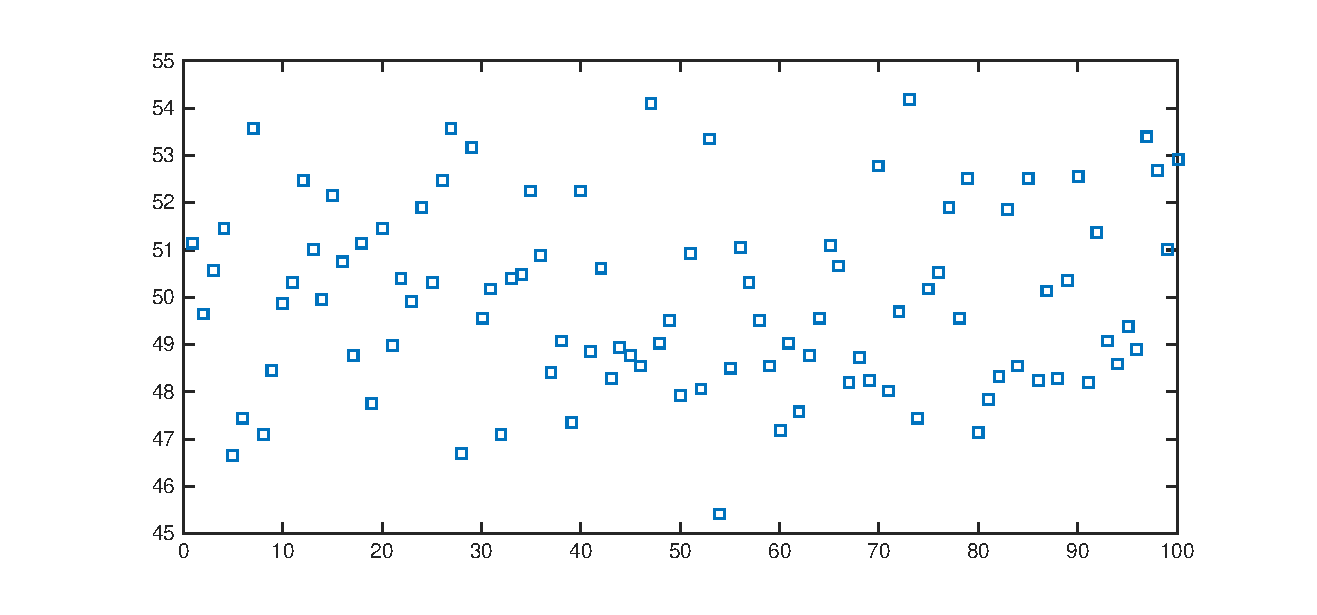
\includegraphics[width=0.8\textwidth]{math_comp.eps}
            \label{fig:root2}
        \end{figure}

}
\subsection{算數平均}
\frame{
\frametitle{巴比倫人的方法}
紀元前三百年(戰國時期)
$$\hat{x}=\frac{1}{100}\sum_{i=1}^{100} y_i$$
}
\subsection{最小平方法}
\frame{
\frametitle{Legendre 及 Gauss}
西元1806,1809年\\
\bigskip
假設 $x$ 為A女真正的體重,$y_i-x$ 代表第 $i$ 次的測量誤差\\
A女體重的最小平方估計為
$$\hat{x}_{LS}\triangleq \min_x \sum_{i=1}^{100} (y_i-x)^2$$

}

\subsection{最大概似函數}
\frame{
\frametitle{Bernoulli}
西元1777年\\
\bigskip
假設 $p(y_1,y_2,\cdots,y_{100}|x)$ 為量測值的條件式聯合機率密度函數,
A女體重的最大(對數)概似估計為
$$\hat{x}_{ML}\triangleq \max_x \hspace{0.2cm}\log p(y_1,y_2,\cdots,y_{100}|x)$$

}

\subsection{貝氏估計}
\frame{
\frametitle{Bayes}
西元1763年\\
\bigskip
提出貝氏定理:$\hspace{2cm}p(x|y)=\frac{p(y|x)p(x)}{p(y)}$\\
\bigskip

A女體重的貝氏估計(或稱 Maximum A Posteriori, MAP 估計)為
$$\hat{x}_{MAP}\triangleq \max_x \hspace{0.2cm}\log p(x|y_1,y_2,\cdots,y_{100})$$
}

\frame{
\frametitle{Gauss}
西元1809年\\
\bigskip
Gauss建立了量測值的模式$\hspace{2cm}\mathbf{y}=x+\mathbf{\epsilon}$\\

並做了以下的假設:\\
\begin{num}
  \item 量測誤差值服從常態分配$\hspace{1cm}\epsilon_i \sim N(0,\sigma^2)$\pause
  \item 量測誤差值 $\epsilon_1,\epsilon_2,\cdots$ 為獨立變數\pause
  \item 未知數 $x$ 為均等分配(意即,對 $x$ 一無所知)
\end{num}
}

\frame{
Gauss得到以下結論\\
\bigskip
$$\hat{x}_{LS}=\hat{x}_{ML}=\hat{x}_{MAP}=\frac{1}{100}\sum_{i=1}^{100} y_i$$

\bigskip 奠定最小平方法的立論基礎,更說明了平均數的內涵。
}

\section{迴歸分析}
\frame{
\frametitle{問題2}
已知 20 個人的體重資料,要預測第21人的體重?

        \begin{figure}[h]
            \centering
            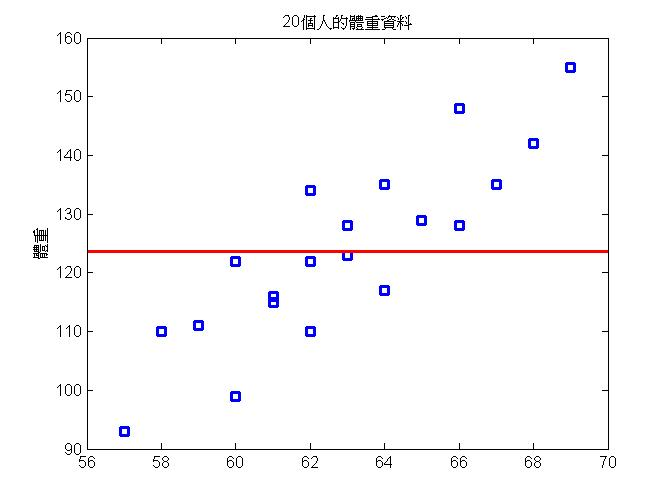
\includegraphics[width=0.6\textwidth]{math_comp_1_1.jpg}
            \label{fig:data1}
        \end{figure}

}
%\subsection{更多的資訊}
\frame{
\; 加入身高資料,對預測有幫助嗎?可以從一個人的身高預測其體重?

迴歸分析:
$$Y=\beta_0+\beta_1X+\alert{\epsilon}$$
\begin{table}[h]
    \centering
 %   \extrarowheight=2pt
    \begin{tabular}{cc}
    \hline
    體重(Y)	& 身高(X)     \\\hline
    93    			& 57            \\
    110    		& 58              \\
    99    			& 60              \\
    112    		& 60              \\
    $\vdots$ & $\vdots$ \\\hline
    \end{tabular}\hspace{10pt}
\end{table}
}

\frame{
\;計算聯立方程式(System of Linear Equations)的解:$\beta_0,\beta_1$


\begin{eqnarray*}
  93 		&=& \beta_0+57\beta_1 \\
  110 	&=& \beta_0+58\beta_1 \\
  99 		&=& \beta_0+60\beta_1 \\
  112 	&=& \beta_0+60\beta_1 \\
  \vdots &=& \vdots
\end{eqnarray*}

有解?無解?無限多組解?
}

\frame{
\; 假設 $\hat{\beta}_0,\hat{\beta}_1$為上述聯立方程式的\alert{解},在已知身高($x$)的情況下,體重的預測
$$\hat{y}=\hat{\beta}_0 + \hat{\beta}_1 x$$
}

\section{時間序列}
\frame{
\frametitle{問題3}
已知 $y_1,y_2,\cdots,y_N$ 為 $N$ 筆依時間排序的資料,欲預測尚未發生的第 $N+1$ 筆 $y_{\scriptscriptstyle{N+1}}$

假設:每筆時間資料都與其前 $p$ 筆資料有關,其關係假設為
$$y_n=a_1y_{n-1} + a_2y_{n-2} + \cdots + a_py_{n-p}$$
}

\frame{
\; 計算聯立方程式(System of Linear Equations)的解:$a_1,a_2,\cdots,a_p$
$$
\begin{array}{lllllllll}
  y_{p+1} & = & a_1y_{p} & + & a_2y_{p-1} & + & \cdots & + & a_py_{1} \\
  y_{p+2} & = & a_1y_{p+1} & + & a_2y_{p} & + & \cdots & + & a_py_{2} \\
  \vdots  &  &  &  &  & \vdots &  &  &  \\
  y_{\scriptscriptstyle{N}} & = & a_1y_{\scriptscriptstyle{N-1}} & + & a_2y_{\scriptscriptstyle{N-2}} & + & \cdots & + & a_py_{\scriptscriptstyle{N-p}} \\
\end{array}
$$
有解?無解?無限多組解?
}

\frame{
\; 假設 $\hat{a}_1,\hat{a}_2,\cdots,\hat{a}_p$為上述聯立方程式的\alert{解},則未知資料 $y_{\scriptscriptstyle{N+1}}$ 的預測為

$$\hat{y}_{\scriptscriptstyle{N+1}}=\hat{a}_1y_{\scriptscriptstyle{N}} + \hat{a}_2y_{\scriptscriptstyle{N-1}} + \cdots + \hat{a}_py_{\scriptscriptstyle{N-p+1}}$$
}
\section{最大概似函數}
\frame{
\frametitle{問題4}
\; 假設 $X$ 為一個服從多項分配的變數, $X\sim M(N,\theta_1,\theta_2,\theta_3)$, $\theta_1+\theta_2+\theta_3=1$

已知 $N=10$ 次的試驗中,這三項的次數分別為 $2,3,5$,如何對母體的參數 $\theta_1,\theta_2,\theta_3$ 做\alert{最好}的估計?
}

\frame{
\;假設 $N=Z_1+Z_2+Z_3$,概似函數寫成

$$L(\bf{\theta})=\left( \begin{array}{c}
                         N \\
                         Z_1Z_2Z_3
                       \end{array}\right)\theta_1^{Z_1}\theta_2^{Z_2}\theta_3^{Z_3}
 $$

\bigskip
最大概似函數的參數估計:$\max_{\bf{\theta}}L(\bf{\theta})$

\begin{eqnarray*}
  \frac{\partial L(\bf{\theta})}{\partial\theta_1} &=& 0 \\
  \frac{\partial L(\bf{\theta})}{\partial \theta_2} &=& 0
\end{eqnarray*}


}

\section{線性代數的角色}
\frame{
\frametitle{Matrix Representation}
$$A\bf{x}=\bf{b}$$
where
$$A=\left[ \begin{array}{cccc}
             a_{11} & a_{12} & \cdots & a_{1n} \\
             a_{21} & a_{22} & \cdots & a_{2n} \\
             \vdots & \vdots & \ddots & \vdots \\
             a_{m1} & a_{m2} & \cdots & a_{mn}
           \end{array}
 \right],\bf{x}=\left[ \begin{array}{c}
                         x_1 \\
                         x_2 \\
                         \vdots \\
                         x_n
                       \end{array}
  \right],\bf{b}=\left[\begin{array}{c}
                         b_1 \\
                         b_2 \\
                         \vdots \\
                         b_m
                       \end{array}
   \right]$$
}
\end{document}

